\chapter{Long Travel Manual Screen}
\section{Overview}\paragraph*{The}\textbf{Long Travel} manual screen (Figure 6.1) provides the Operator access to control the \textbf{Long Travel} axis while in \textit{Hand} mode. The Operator is able to initiate a homing function or move to limit, and there are indicators for \textbf{At Home} and \textbf{At Limit}, plus for while in motion. Navigation is possible to the main \textbf{Manual} screen, the \textbf{Cut Program} screen, both the \textbf{Vertical Axis} and \textbf{Cross Travel Axis} manual screens, and of course the \textbf{Main} operation screen.
\begin{figure}
	\centering
	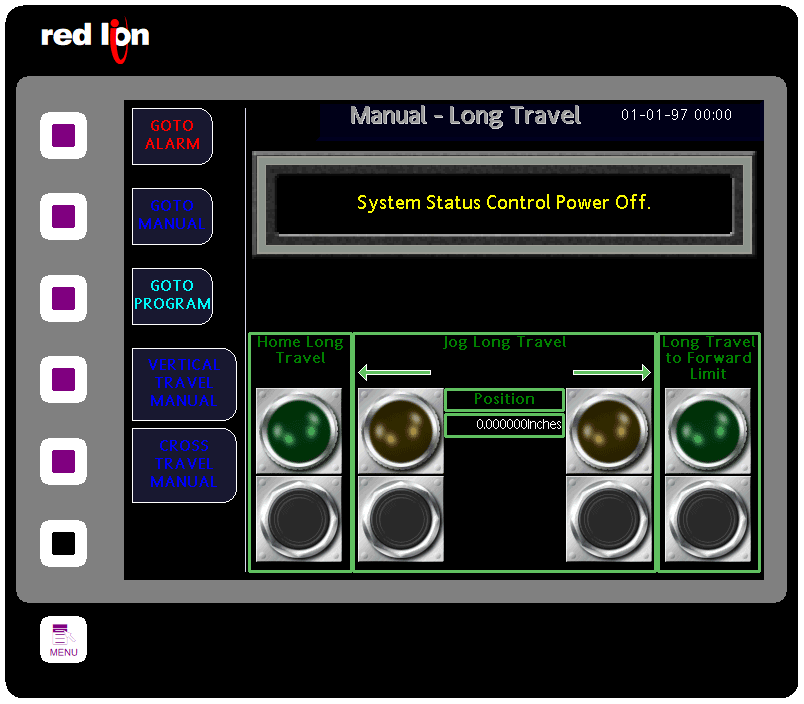
\includegraphics[width=0.5\linewidth]{screen-captures/manual/long-manual}
	\caption{Long Travel Manual Screen}
	\label{fig:manual-long-screen}
\end{figure}
\section{Details}\paragraph*{The}\textbf{Long Travel Manual} screen details are divided into the following categories ...
\begin{list}{$\diamond$}{}
	\item \textbf{Screen Navigation}
	\item \textbf{Long Travel Home and To Limit}
	\item \textbf{Long Travel Control}
\end{list}
\pagebreak
\subsection{Screen Navigation}
\paragraph*{Is}performed by using the programmable Function Keys (FKeys) located down the left hand side of the OI Terminal (refer to Figure 6.2). The Operator may navigate to the following screens ...
\begin{list}{$\diamond$}{}
	\item \textbf{GOTO ALARM} Navigate to Alarm Screen.
	\item \textbf{GOTO MANUAL} Navigate to Manual Screen.
	\item \textbf{GOTO PROGRAM} Navigate to Cut Program Screen.
	\item \textbf{VERTICAL MANUAL} Navigate to Vertical Manual Control Screen.
	\item \textbf{LONG AXIS MANUAL} Navigate to the Long Axis Manual Control Screen.
\end{list}
\begin{figure}
	\centering
	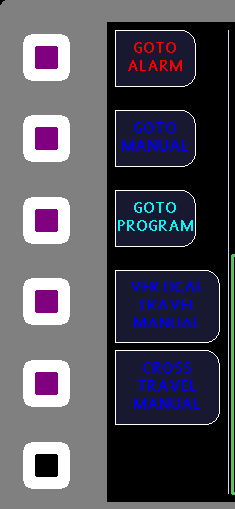
\includegraphics[width=0.2\linewidth]{screen-captures/manual/long-manual-nav}
	\caption{Long Travel Manual Screen Navigation}
	\label{fig:manual-long-screen-nav}
\end{figure}
\paragraph{\textbf{\LARGE \textcolor{blue}{i}}}
The Menu Key located on the terminal at the lower left below the FKey's, will return the Operator to the Main Screen, from all other screens.\\
\begin{minipage}{4cm}
	\begin{picture}(20,70)
		
\includegraphics[width=.5\linewidth]{screen-captures/menu}
	\end{picture}
\end{minipage}\begin{minipage}[]{11cm}
	\paragraph{\textbf{\LARGE \textcolor{blue}{i}}} The Menu Key is pictured as it looks on the Terminal.
\end{minipage}
\pagebreak
\subsection{Long Travel Home and To Limit}\paragraph*{Home and To Limit}Functions are the stand alone homing and move to limit routines for the \textbf{Long Travel} axis. There is a \textbf{Control} pushbutton to initiate the homing/to limit function and an \textbf{Indicator} pilot light to indicate when the \textbf{Long Travel} axis is in the \textbf{Home/Limit} position and has completed a homing/move to limit function. On the saw the \textbf{Long Travel} axis has it's \textbf{Home} position at the travel limit sensor target furthest to the left when facing the Control Panel. A homing function will initiate a homing program in the master drive of the axis to home the axis. While a move to limit function will move the Long axis towards it's forward limit target. 
\begin{figure}
	\centering
	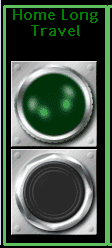
\includegraphics[width=.2\linewidth]{screen-captures/manual/long-manual-home}
	\caption{Long Travel Manual Home Function}
	\label{fig:long-manual-home}
\end{figure}
\begin{figure}
	\centering
	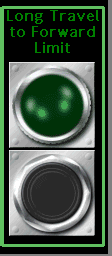
\includegraphics[width=.2\linewidth]{screen-captures/manual/long-manual-tolim}
	\caption{Long Travel Manual To Limit Function}
	\label{fig:long-manual-tolim}
\end{figure}
\pagebreak
\subsection{Long Travel Positioning}
\paragraph*{}Figure 5.4 shows the \textbf{Long Travel Command} function. The function is made up of a pushbutton to command \textbf{Long Travel Forward} with a corresponding \textbf{Indicator} pilot light that indicates motion commanded but not complete. There is also a related \textbf{Long Travel Reverse} pushbutton and \textbf{Indicator}. Finally, there is a position feedback display area which shows the current axis position in inches. This function is available in \textit{Hand} mode and is intended for use by the Operator during Machine Setup and Maintenance activities. This function uses inputs to the Master Drive of the axis to jog in either direction according to the parameters programmed into the drive for jogging.
\begin{figure}
	\centering
	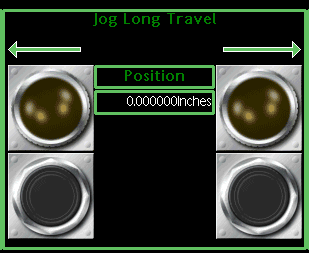
\includegraphics[width=.2\linewidth]{screen-captures/manual/long-manual-command}
	\caption{Cross Travel Manual Command}
	\label{fig:long-manual-command}
\end{figure} 
\paragraph{\textbf{\LARGE \textcolor{blue}{i}}}The position feedback should be considered invalid if the axis has not been homed yet. A Home command must be initiated in order to ensure positional accuracy and repeatability.
